% UM-SJTU JI PHYS1600J Project Template based on RevTeX 4.2 Template.
\documentclass[reprint]{revtex4-2}

% You can add packages here.
\usepackage{lipsum}
\usepackage{graphicx}
\usepackage{geometry}
\usepackage{subfigure}
\usepackage{amsfonts,amsmath,amssymb}
\usepackage{enumerate}
\usepackage{dcolumn}
\usepackage{bm}
\usepackage[colorlinks,citecolor=black,urlcolor=black]{hyperref}
\hypersetup{colorlinks=true,linkcolor=black}
\usepackage[mathlines]{lineno}

% Additional Packages
\usepackage{float}  % Float

\begin{document}

\title{Problem B\\ Optimizing Hovercraft Design: Balancing Propulsion, Lift, and Stability}

\author{Yingzeng Li}
\email{2024lyz@sjtu.edu.cn}
\author{Leqi Tang}
\email{luckysugar@sjtu.edu.cn}
\author{Zirui Wang}
\email{wzr0831@sjtu.edu.cn}
\author{Zijie Qu}
\email{Correspondence: zijie.qu@sjtu.edu.cn}
\affiliation{UM-SJTU Joint Institute, Shanghai Jiao Tong University, Shanghai 200240, China}

\begin{abstract}
Our study investigates the optimal design of hovercraft based on our definition of "optimal" with a set scenario, specifically focusing on air cushion vehicles (ACVs). By analyzing existing ACV prototypes, we decompose the system into key components that vary across designs. Our principle is to optimize each of the component by comparing existing model or through theoretical analysis, aiming to reach global optimization with the combination of local optimization. For each component, we will develop physical models to characterize the dynamic behavior of the reality and figure out optimal condition. Notably, we'll integrate the modeling part with result of each model so as to maintain the coherence of the analysis process. In particular, a simplified model of the fan system—comprising both propulsion and lift fans—is constructed, along with a representation of the cushion pressure zone, which compose the main part of the hovercraft. Furthermore, we compare vehicle performance on land and over water to assess stability under different surface conditions. Key findings indicate that optimal fan positioning can mitigate angular momentum effects, while the use of multiple fans may incur diminishing returns due to increased energy losses. Structural parameters such as overall length and cushion geometry are also shown to significantly influence dynamic behavior.  Overall, this research offers theoretical insights into the design optimization of amphibious hovercraft and supports more informed design decisions in practical engineering contexts.

\begin{description}
    \item[Keywords] Hovercraft, Air Cushion Vehicle, Dynamics, Fan systems, Design Optimization
\end{description}

\end{abstract}

\maketitle

\section{Introduction}

\subsection{Background}

Hovercraft are unique transportation platforms capable of traversing both terrestrial and aquatic environments by riding on a cushion of pressurized air. Their amphibious capability arises from the fundamental principle of reducing ground contact through an air cushion, thereby minimizing friction and enabling smooth travel over irregular or soft surfaces. This makes them particularly valuable in situations such as military operations.

The design of a hovercraft involves complex trade-offs between lift generation, propulsion efficiency, and structural stability. Central to its operation is the lift system, which maintains a stable air cushion by balancing incoming air pressure and leakage beneath the skirt. In amphibious applications, additional considerations arise, including changes in load distribution and surface interaction. The control and stability of the craft are further influenced by the location and number of fans, the geometry of the hull and skirt, and the characteristics of the operating surface.

As demand grows for agile and versatile vehicles in both civilian and defense sectors, optimizing hovercraft design becomes increasingly critical. Prior research has focused on various aspects of hovercraft dynamics, yet a unified framework connecting power constraints, pressure distribution, and performance across multiple terrains remains limited. This study addresses that gap by developing and analyzing physical models tailored for amphibious ACVs, laying foundation for improved design strategies under real-world operational constraints.

\begin{figure}[H]
  \centering
  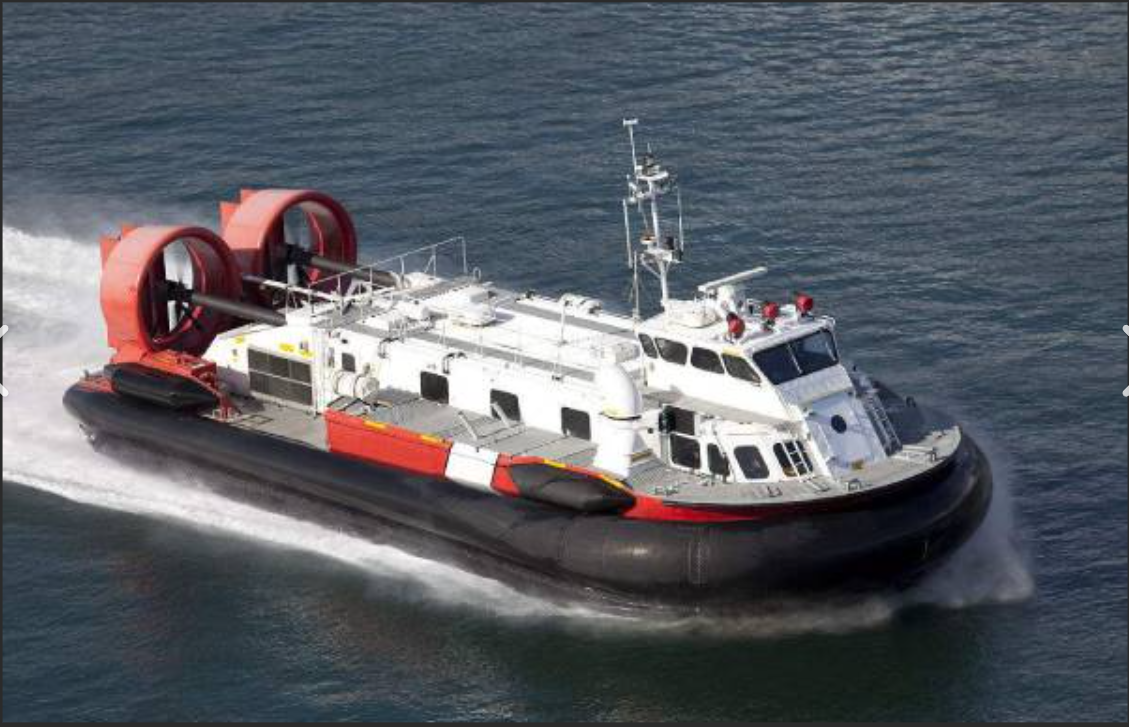
\includegraphics[width=0.5\textwidth]{images/Hovercraft.png}
  \caption{Hovercraft\cite{hovercraftImage}}
  \label{fig:Hovercraft}
\end{figure}

\subsection{Problem Restatement}
This project aims to determine the optimal design of an air cushion vehicle (ACV) powered by a single fixed-output engine. The key challenge is to decide the best configuration and placement of the fan system. Also, this project needs to optimize the efficiency on both water and ground surface.

Ultimately, the goal is to identify fan arrangements and structural parameters that maximize efficiency and stability that applies to various ship types.

\subsection{The Definition of Optimal Arrangement}

In terms of the definition of "optimal", we need first to clarify the scenario of the usage of hovercraft. According to \textit{Hovercraft Technology, Economics and Applications}~\cite{amyot2013hovercraft}, the main application of hovercraft is to carry people or transport cargo. Aiming to optimize the function of the hovercraft in the context of this application, we plan to judge the term "optical" in the following way: 
\begin{itemize}
\item the model can provide maximum amount of power to the propulsion fan
\item it can remain steady in process of voyage 
\item it can provide passengers with highest level of comfort if other condition remain optimal
\end{itemize}
\section{Assumptions}

\textbf{Assumption 1:} The power of the engine can be distributed to propulsion fan and lift fan without any loss.

\textbf{Justification:} Ignoring transmission losses simplifies power allocation calculations, allowing focus on optimizing fan efficiency in practical designs.

\textbf{Assumption 2:} The hovercraft won't contact with water or ground during the voyage.

\textbf{Justification:} Hovercraft operate on an air cushion to minimize friction. Assuming no contact aligns with real-world characteristic.

\textbf{Assumption 3:} Temperature change won't cause any effect to the whole system

\textbf{Justification:} Assuming constant temperature avoids complex thermal effects on air density or materials, reasonable for short-term operations in stable environments.

\textbf{Assumption 4:} The effect of the air is limited to air friction, turbulent flow and density inconsistency is negligible. 

\textbf{Justification:} Ignoring turbulence and density variations simplifies aerodynamic calculations, focusing on air friction, which dominates in practical hovercraft skirt designs.

\textbf{Assumption 5:} The center of mass of the hovercraft is at its geometric center

\textbf{Justification:} Assuming a centered mass simplifies stability and torque calculations, reasonable for symmetrical designs, facilitating practical dynamic analysis.

\section{Notations}
The notation table is listed following.
\begin{table*}

\caption{\label{Notation Table}Notation table.}
\begin{ruledtabular}
\begin{tabular}{cc}
\textbf{Symbols} & \textbf{Description}\\
\toprule

$A$ & fan flow area \\
$b$ & breadth of air cushion \\
$C$ & perimeter of craft\\
$C_D$ & profile drag coefficient, based on cushion area \\
$C_L$ & coefficient of aerodynamic lift, based on cushion area \\
$F = \frac{V}{\sqrt{lg}}$ & Froude number \\
$h_0$ &  height of air gap or the gap of peripheral Jet
 \\
$h $ &  height of the hovercraft from the ground  \\
$h_1$ &  height of the hovercraft \\
$I$ & the amplitude of sound wave \\
$J$ & momentum flux per unit length of jet \\
$K$ & coefficient of discharge, for gap at periphery of plenum-chamber craft \\
$K^{'}=\frac{Chp^{\frac{3}{2}}_{c}}{2\rho^{\frac{1}{2}}(1+\cos{\theta})}$ &  dimensionless parameter to simplify calculation\\
$k = \frac{q}{p_c}$ & cushion pressure parameter \\
$L_1$ & distance of the lift fan to COM \\
$L$ & length of hovercraft \\
$L_0$ & estimated sound power level (dB) of
the fan \\
$l$ & length of cushion\\
$m$ & mass of craft \\
$P_0$ & fixed power output from one single engine \\
$P_L$ & lifting fan power \\
$P_M$ & power to overcome momentum drag \\
$P_T$ & total power \\
$p_c$ & pressure in air cushion, relative to atmosphere \\
$p_J$ & mean total pressure of jet at nozzle exit, relative to 
atmosphere \\
$p_0$ & the pressure of atmosphere \\
$Q$ & volume flow per unit time in lifting jets \\
$q = \frac{1}{2}\rho v_f^2$ & dynamic pressure associated with forward speed \\
$R$ & wave drag \\
$S$ & cushion area \\
$t$ & thickness of jet at nozzle exit \\
$V$ & the volume of air exiting the jet \\
$v_f$ & forward speed of craft \\
$v_0$ & the speed of gas escape from air cushion to atmosphere \\
$v_{jet}$ & the gas speed of jet at nozzle exit\\ 

$x = \frac{(1+\cos\theta)t}{h}$ & dimensionless parameter \\
$z$ & the height of center of propulsion fan \\
$\alpha$ & angle defining attitude of craft \\

$\theta$ & inclination of jet to horizontal at nozzle exit \\
$\eta$ & intake efficiency \\
$\rho$ & density of air (assumed constant) \\
$\rho_w$ & density of water \\
$\sigma = p_c/\rho_w l g$ & dimensionless pressure parameter \\

\end{tabular}
\end{ruledtabular}
\end{table*}


\section{Theoretical Model and Result}
In this section, we will systematically decompose the optimization objectives into manageable, smaller components to facilitate a structured and efficient approach to model refinement. The primary strategy involves optimizing each sub-component of the model either independently or by leveraging the outcomes of previously optimized components. 

Additionally, all optimization results are consolidated and presented in this section to uphold analytical completeness, providing a clear, comprehensive view of how individual improvements enhance overall model performance. This organization supports robust, iterative refinement aligned with the study's objectives.
\subsection{Ideal Model of the Cross-section of Hovercraft}
\label{sec:model}

In this section, we'll decide the best design of the cross-section of the hovercraft between two mainstream designs based on the evaluation of energy efficiency and stability.

In designing the cross-section of a hovercraft, two mainstream approaches are commonly considered~\cite{mair1964physical}.  The first approach adopts a simplified geometric design with symmetrical "L"-shaped supports and a centralized fan. The second approach involves a design with a complex curved structure, featuring a fan that directs airflow downward and outward through intricate paths, as indicated by the angle $ \theta $. 
\begin{enumerate}
    \item the gas is incompressible
    \item the side wall of the hovercraft is very narrow such that it can be modeled as a short pipe 
    \item the viscosity of the air is negligible
    \item the air flow is steady
\end{enumerate}

Then we can simplify the model of the cross-section using the following figure, whose aerodynamics design is highly consistent with two mainstream model. Notably, the gas comes from all around the bottom of the hovercraft instead of just being emitted from one whole, which will be beneficial to the models in the following parts. Also, the fan above is just to give an intuitive sense, the detailed number of fans will be discussed in the following parts.

\begin{figure}[H]
  \centering
  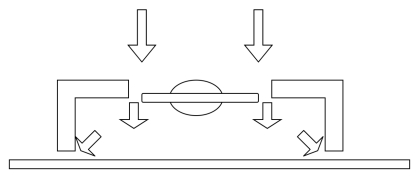
\includegraphics[width=0.5\textwidth]{images/PlenumChamber.jpg}
  \caption{Plenum Chamber}
  \label{fig:Plenum Chamber}
\end{figure}

\begin{figure}[H]
  \centering
  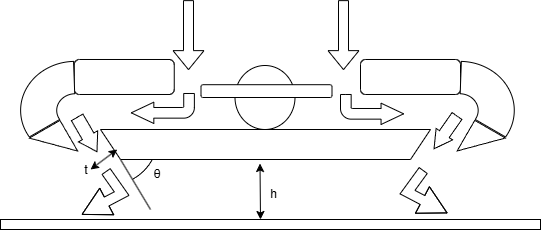
\includegraphics[width=0.5\textwidth]{images/PeripheralJet.jpg}
  \caption{Peripheral Jet}
  \label{fig:PeripheralJet}
\end{figure}


Then, by using Bernoulli’s equation, the flow rate can be calculated for both of two models.\\
For an orifice ($S\!=\!h_0\!\times\!L$) with pressure drop $\!p_c\!$:
\begin{enumerate}
\item Bernoulli formula gives that:
\begin{equation}
p_c = \frac{1}{2}\rho v_0^2
\end{equation}
where $p_c$ is the pressure relative the pressure of atmosphere.
\item Solve for exit velocity:
\begin{equation}
v_0 = \sqrt{\frac{2p_c}{\rho}}
\end{equation}

\item Flow rate:
\begin{equation}
Q = S \cdot v_0 = h_0 \cdot L \cdot \sqrt{\frac{2p_c}{\rho}}
\end{equation}
where $h_0$ can be either the height of air gap or the gap width of Peripheral Jet, which in this condition is $t$ in FIG.3.
\end{enumerate}

That is to say, flow rate $Q$ is proportional to the height of air gap in the model of Plenum Chamber. As result, The air supply system's power consumption remains excessive unless the boundary gap width is significantly reduced, resulting in considerable amount of power. In maritime applications like air-cushion vessels operating in rough seas, maintaining consistent gas flow is critical. When the orifice size remains fixed, the system exhibits inherent stability even under wave-induced hull vibrations. Thus, we choose the model of Peripheral Jet to be the best model of cross-section.

\subsection{Principles of Air Cushion Mechanics}
\label{sec:ACM}
Having established the peripheral jet configuration as the optimal cross-sectional design for the hovercraft lift system, we now examine the fundamental physical mechanisms governing the supporting air cushion. A precise understanding of the momentum exchange between the jet flow and the high-pressure region beneath the hull is critical for evaluating lift performance, ensuring stability, and informing skirt design.

To this end, we adopt the momentum-conservation-based modeling framework proposed by Whitham, which treats the air cushion as an open control volume bounded by the hull, flexible skirt, and ambient atmosphere. This approach facilitates the derivation of a quantitative relationship between the input jet momentum and the resulting cushion pressure, accounting for geometric characteristics and empirical correction factors.

\begin{figure}[H]
  \centering
  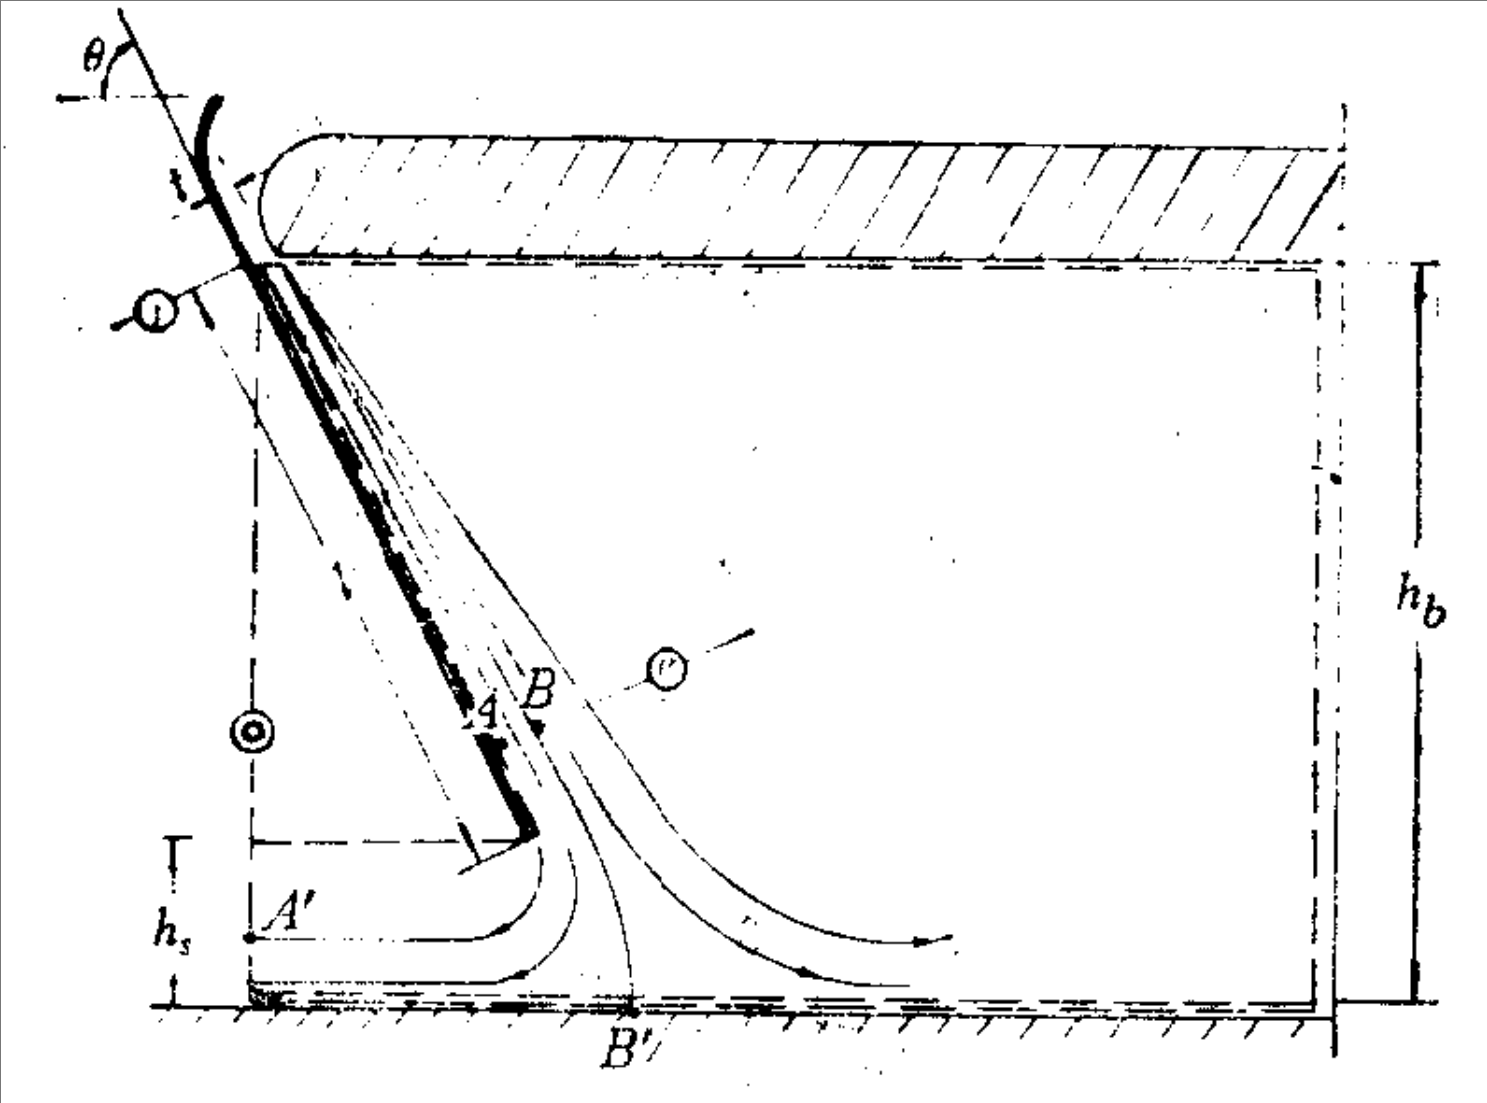
\includegraphics[width=0.5\textwidth]{images/JetModel.png}
  \caption{Schematic of the planar jet model}
  \label{fig:JetModel}
\end{figure}

As illustrated in Figure~\ref{fig:JetModel}, we analyze the streamwise momentum flux of a steady, planar nozzle jet under the following assumptions:
\begin{enumerate}
    \item The flow is steady and two-dimensional, with negligible variation in the spanwise direction.
    \item The velocity is uniform across the jet cross-section, and the jet exits the nozzle at a constant speed \( v_{jet} \).
    \item The jet maintains constant density \( \rho \) and has an effective thickness \( t \), representing the finite jet width per unit depth in the two-dimensional approximation.
    \item The control surface is aligned with the flow direction so that only streamwise momentum is considered.
\end{enumerate}

Over a small time interval \( \Delta t \), the volume of air exiting the jet is given by:
\begin{equation}
V = v_{jet} t \Delta t,
\end{equation}
where \( t \) has units of \( \mathrm{m}^2 \), representing cross-sectional area per unit depth.

The corresponding streamwise momentum flux is:
\begin{equation}
J = \frac{M v_{jet}}{\Delta t},
\end{equation}
where \( M = \rho V \) is the mass of fluid crossing the control surface during \( \Delta t \). Substituting yields:
\begin{equation}
J = \rho v_{jet}^2 t
\label{eq:momentum flux}
\end{equation}

Assuming the flow is steady, incompressible, and that the elevation difference between the fan and the nozzle exit is negligible, Bernoulli’s equation relates the total pressure \( H \) to the static pressure at the nozzle exit \( p_{\text{jet}} \) as:
\begin{equation}
H = p_{\text{jet}} + \frac{1}{2} \rho v_{\text{jet}}^2.
\end{equation}
Substituting \( v_{\text{jet}}^2 \) into the expression for the momentum flux yields:
\begin{equation}
J = 2 (H - p_{\text{jet}}) t.
\end{equation}

Here, \( H = p_J + \frac{p_0}{2} \), as the surrounding air is assumed to be moving with a dynamic pressure of \( \frac{p_0}{2} \). Moreover, since \( p_{\text{jet}} - p_0 = p_c \), the momentum flux can also be written as:
\begin{equation}
J = (2p_J - p_c) t. \label{eq:J_p0}
\end{equation}

This relation is essential for fan system design: to maintain a sufficient cushion pressure, the fan must deliver a total pressure high enough to sustain the required jet momentum.

At the nozzle exit section \( e \), the total jet momentum flux \( M_j \) is partitioned into two components:
\begin{itemize}
    \item \( M_f \): the momentum flux directed into the cushion region;
    \item \( M_e \): the momentum flux leaking directly into the atmosphere.
\end{itemize}

By conservation of momentum:
\begin{equation}
M_j = M_f + M_e.
\end{equation}

To relate this partition to the skirt geometry, Whitham employs an empirical correlation based on turbulent wall jet studies (Meyer’s formula), expressing the leakage ratio as:
\begin{equation}
\frac{M_e}{M_f} = 2.75 \left( \frac{h_b - h_f}{t \sin \theta} \right) - 0.45,
\end{equation}
where:
\begin{itemize}
    \item \( h_b - h_f \) is the vertical gap between the nozzle exit and the skirt edge;
    \item \( t \sin \theta \) is the vertical thickness of the incoming jet;
    \item 2.75 and \( -0.45 \) are empirically derived constants.
\end{itemize}

This expression enables a direct evaluation of cushion pressure based on geometric and flow parameters. For typical skirt geometries, experimental observations suggest that the leakage and cushion-directed momenta are approximately equal:
\begin{equation}
M_f \approx M_e = \frac{M_j}{2}.
\end{equation}
This approximation simplifies subsequent analysis without significant accuracy loss.

We now consider a vertical momentum balance over a control volume bounded above by the rigid hull, laterally by the inclined skirt, and below by the ambient atmosphere. Applying Newton’s second law in the vertical direction yields:
\begin{equation}
p_{jet} h_b - \int_0^l p \sin \theta \, dl - p_0 h_s = M_f \cos \theta + M_e,
\end{equation}
where:
\begin{itemize}
    \item \( p_c h_b \) is the upward force from the cushion pressure acting on the hull base;
    \item \( \int_0^l p \sin \theta \, dl \) is the vertical pressure force on the inclined skirt of length \( l \) and angle \( \theta \);
    \item \( p_0 h_s \) is the downward force from ambient atmospheric pressure on the skirt exit;
    \item \( M_f \cos \theta \) is the vertical momentum transferred into the cushion;
    \item \( M_e \) accounts for vertical momentum from leakage, including effects due to turbulence and separation.
\end{itemize}

Assuming constant skirt angle and uniform cushion pressure \( p_c \) along the skirt wall, the integral simplifies as:
\begin{equation}
\int_0^l p \sin \theta \, dl = p_c \sin \theta \cdot l = p_c (h_b - h_s),
\end{equation}
where \( h_b - h_s = l \sin \theta \) is the vertical projection of the skirt.

Substituting into the vertical momentum balance and rearranging terms, we obtain:
\begin{equation}
(p_{jet} - p_0) h_f = M_f ( \cos \theta + 1),
\end{equation}
where \( h_f \) represents an effective vertical length that accounts for the base area, skirt projection, and skirt exit geometry.

To express the relation more meaningfully, we define the air cushion pressure relative to atmospheric pressure as \( p_c = p_{\text{jet}} - p_0 \). The momentum balance equation then becomes:
\begin{equation}
    p_c h_f = J ( \cos \theta + 1)
    \label{eq:force_balance}
\end{equation}
In summary, the model begins by estimating the jet velocity and momentum using Bernoulli’s principle. The total momentum is then partitioned into cushion-directed and leaked components. The vertical momentum balance links cushion pressure to this partition, while empirical models relate the momentum distribution to geometric parameters. This framework serves as a predictive tool for evaluating lift capability and optimizing skirt configuration.

\subsection{Comparative Modeling of Centrifugal and Axial Flow Fans}
In this section, we'll consider the best choice of lift fan and propulsion fan among two existing types of fans, namely centrifugal fan and axial flow fan.\\
From the momentum balance equation~\eqref{eq:force_balance} applied to the air cushion,
\[
    p_c h = J(1 + \cos\theta),
\]
where \( p_c \) denotes the cushion pressure relative to atmospheric pressure, \( h \) is the hover height, and \( J \) is the injected momentum flux.

For a hovercraft with fixed geometry—neglecting the mass of the fan and deformation of the skirt—the cushion pressure \( p_c \) must exceed a critical threshold to counterbalance the vehicle’s weight. Consequently, \( p_c \) is primarily determined by the required lift force and can be regarded as an external design constraint imposed on the fan system.

In contrast, the hover height \( h \) is a system response variable that increases with the available momentum flux \( J \). A larger \( h \) enhances ground clearance and contributes to improved dynamic stability, especially on uneven terrain or during motion. Thus, while \( p_c \) ensures the feasibility of lift, the magnitude of \( h \) governs the overall operational performance of the hovercraft.

To achieve a more stable operating condition, the injected momentum flux \( J \) must be sufficiently large to maintain an adequately high hover height \( h \). This requirement, in turn, necessitates a carefully designed and efficient fan system.

\begin{figure}[H]
  \centering
  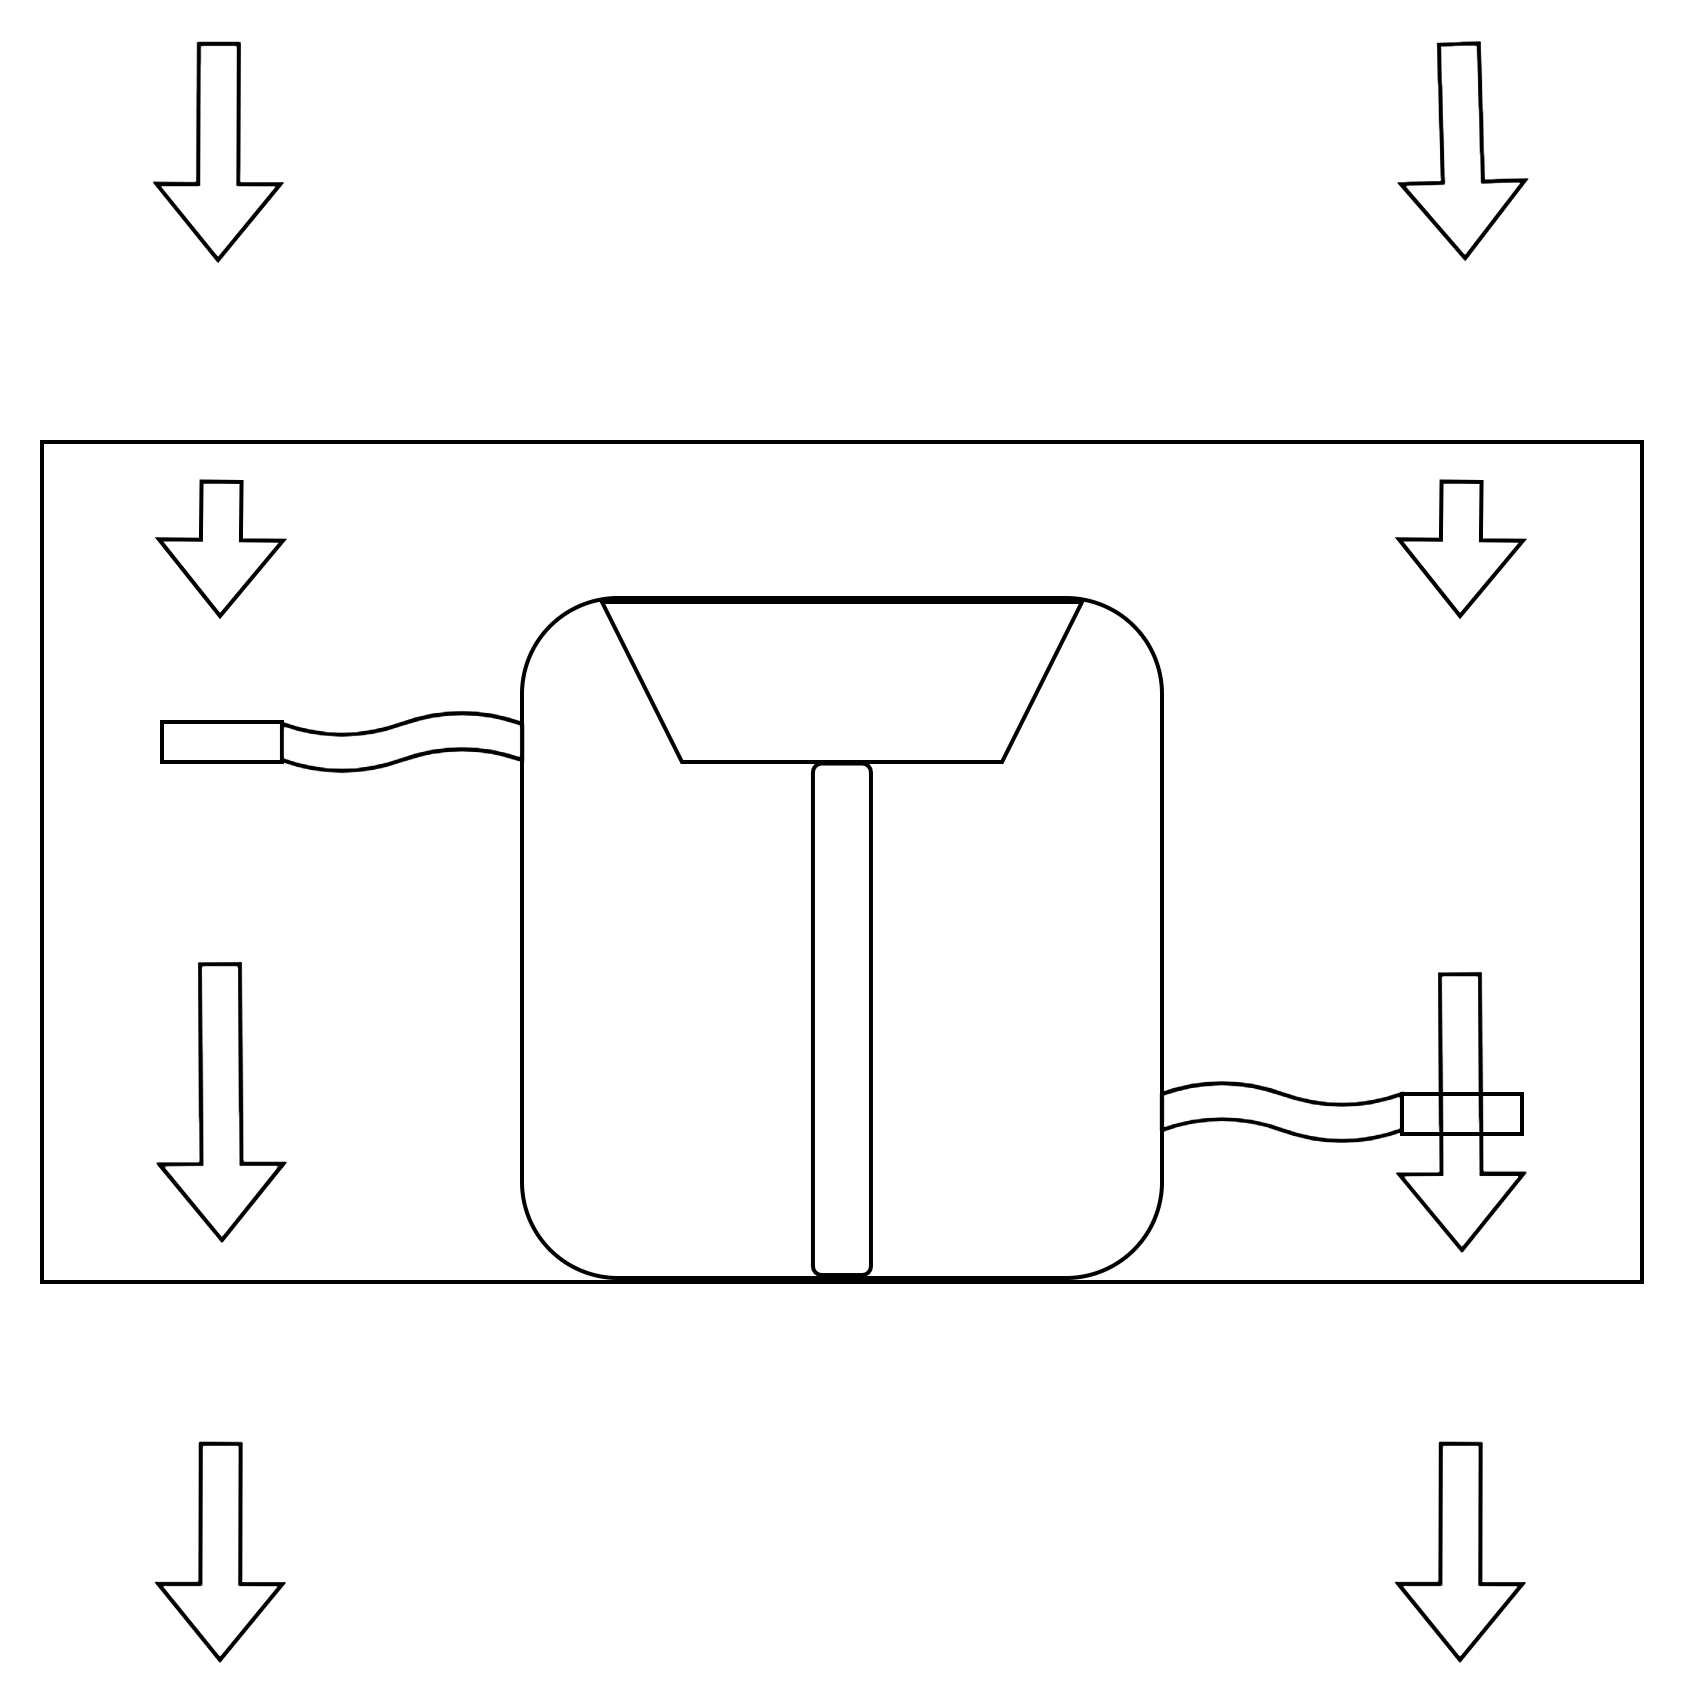
\includegraphics[width=0.5\textwidth, height=0.45\textwidth]{images/FanModel.png}
  \caption{Schematic diagram of the fan model}
  \label{fig:FanModel}
\end{figure}

As illustrated in Fig.~\ref{fig:FanModel}, the fundamental principle of the fan system is to generate a pressure difference between the internal air cushion and the external atmosphere, thereby inducing a volumetric flow that delivers the required momentum flux \( J \). Notably, the length of the arrow in Fig. 5 represents the velocity of the air flow.
The injected momentum flux \( J \) depends on both the volumetric flow rate \( Q \) and the jet velocity \( v_{\text{jet}} \), which are governed by the aerodynamic characteristics of the fan. Assuming a two-dimensional jet of width \( t \), the volumetric flow rate can be expressed as
\begin{equation}
    Q = \rho v_{\text{jet}} t,
\end{equation}
where \( \rho \) is the air density. Substituting this into the definition of momentum flux (cf. equation~\eqref{eq:momentum flux}) yields
\begin{equation} \label{eq:Mj_revisited}
    J = \rho v_{\text{jet}}^2 t = \frac{Q^2}{\rho t}.
\end{equation}

The input power \( P \) required to sustain the air cushion can be estimated as
\begin{equation}
    P = \frac{\Delta p \cdot Q}{\eta},
\end{equation}
where \( \Delta p \approx p_c \) is the pressure rise across the fan, and \( \eta \) denotes the fan efficiency. This expression highlights two critical performance parameters: the pressure rise \( \Delta p \) and the volumetric flow rate \( Q \).

Notably, for a given nozzle width \( t \), the momentum flux \( J \) scales quadratically with the volumetric flow rate \( Q \), underscoring the aerodynamic efficiency benefits of high-throughput fan configurations.

In the following, two primary fan models are presented to compare the relationship between \( p_c \) and \( Q \). Combining these with equation~\eqref{eq:force_balance} enables solving for the hover height \( h \).


\subsubsection{Axial Fan Model}

The axial fan is characterized by its airflow direction, which is predominantly parallel to the fan shaft, i.e., along the axial direction. This feature enables efficient transport of large volumes of air with relatively low pressure rise, making axial fans suitable for applications requiring high flow rates but moderate pressure.


\begin{figure}[H]
  \centering
  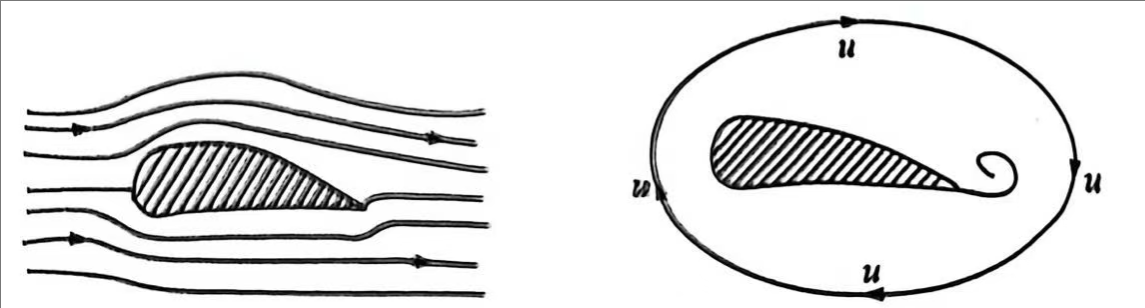
\includegraphics[width=0.5\textwidth]{images/AxialFan.png}
  \caption{Axial Fan Model}
  \label{fig:Axial Fan Model}
\end{figure}

\begin{figure}[H]
  \centering
  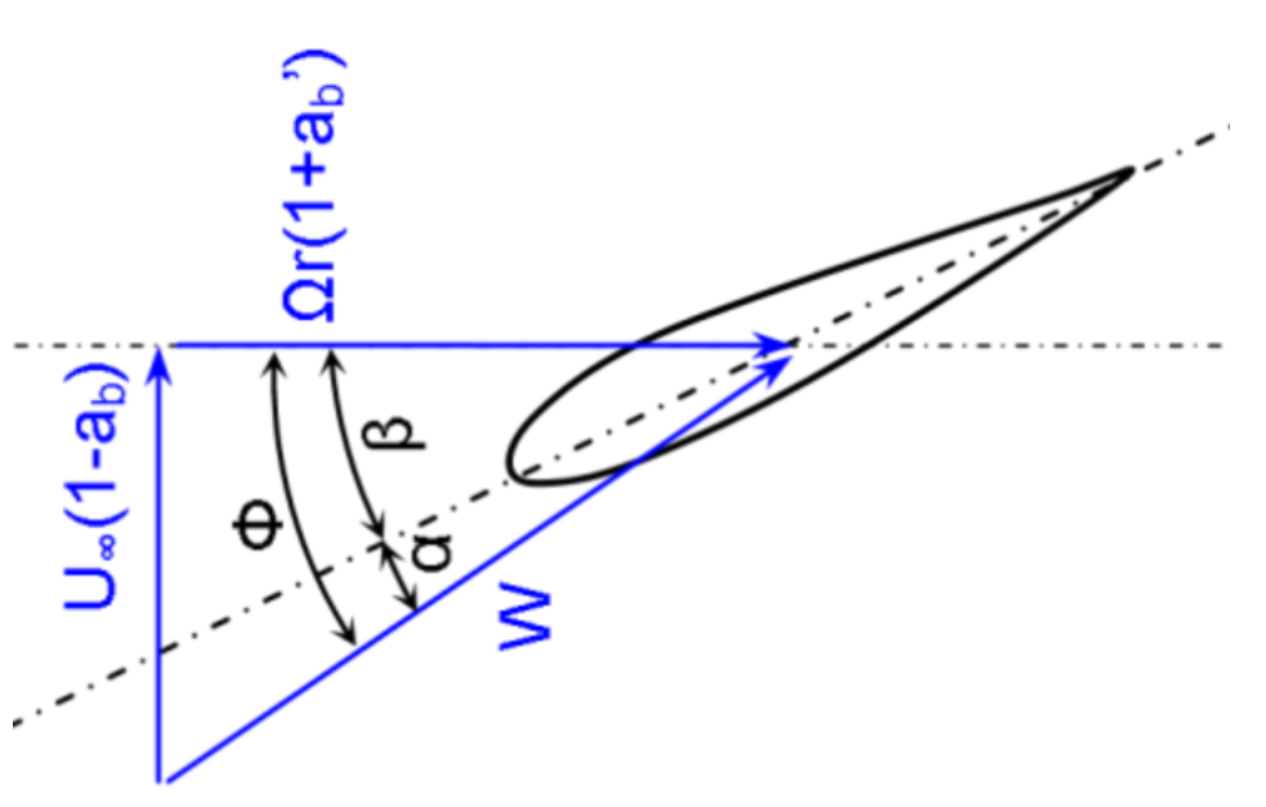
\includegraphics[width=0.5\textwidth]{images/blade.png}
  \caption{Blade Element Model}
  \label{fig:Blade Element Model}
\end{figure}

The axial fan model is developed by analyzing local flow at each blade element under the following simplifying assumptions:
\begin{itemize}
    \item Flow is primarily axial with negligible radial velocity components.
    \item Each blade behaves as an airfoil generating lift and drag forces.
    \item Viscous losses are initially neglected and later accounted for via a global efficiency coefficient \( \eta \).
\end{itemize}

At a blade element located at radius \( r \), the characteristic velocities are:
\[
\begin{array}{ll}
    v_a = \frac{Q}{A}  & \text{axial velocity} \\
    v_t = \omega r     & \text{tangential velocity} \\
    v_r = \sqrt{v_a^2 + v_t^2} & \text{relative inflow velocity}
\end{array}
\]

The inflow angle \( \phi \) and angle of attack \( \alpha \) are given by
\begin{align}
    \tan \phi &= \frac{v_a}{v_t} = \frac{Q}{\omega r A}, \\
    \alpha &= \theta - \beta,
\end{align}
where \( \beta \) is the blade pitch angle.

Lift and drag forces on a blade element of chord length \( c \) are
\begin{align}
    dL &= \frac{1}{2} \rho v_r^2 C_L(\alpha) c \, dr, \\
    dD &= \frac{1}{2} \rho v_r^2 C_D(\alpha) c \, dr,
\end{align}
where \( C_L \) and \( C_D \) are lift and drag coefficients as functions of \( \alpha \).

These forces resolve into axial and tangential components:
\begin{align}
    dF_a &= dL \cos \phi - dD \sin \phi, \\
    dF_t &= dL \sin \phi + dD \cos \phi.
\end{align}

The differential pressure rise from the axial force of \( N \) blades over an annular ring \( 2 \pi r \, dr \) is
\begin{equation}
    d(\Delta p) = \frac{N \cdot dF_a}{2 \pi r \, dr}.
\end{equation}

Integrating over the blade span yields the total pressure rise \( \Delta p \). For engineering estimates, assuming small angle of attack (\( \alpha \approx 5^\circ \)) and uniform induced velocity, the axial pressure rise can be approximated as
\begin{equation}
    \Delta p \approx \rho v_a v_\theta,
\end{equation}
where the induced circumferential velocity is approximated by
\begin{equation}
    v_\theta \approx k \omega r,
\end{equation}
with empirical coefficient \( k \approx 0.2 \).

Evaluated at the blade tip \( r = R \) and substituting \( v_a = Q/A \), this gives
\begin{equation}
\boxed{\Delta p_{\text{axial}} \approx 1.2 \eta \rho \omega R \frac{Q}{A}},
\end{equation}
where \( \eta \) accounts for aerodynamic efficiency losses.

\textbf{Validation(SKMR-1 axial fan):}~\cite{yun1990hovercraft}
\begin{itemize}
    \item Fan radius \( R = 0.99\, \mathrm{m} \)
    \item Hub radius \( r_\mathrm{hub} = 0.3\, \mathrm{m} \)
    \item Rotational speed \(\omega = 125.66\, \mathrm{rad/s} \)
    \item Flow rate \( Q = 73.6\, \mathrm{m^3/s} \)
    \item Total pressure rise \( \Delta p = 2873\, \mathrm{Pa} \)
    \item Efficiency \( \eta = 0.79 \)
\end{itemize}

Calculate flow area:
\[
A = \pi (R^2 - r_\mathrm{hub}^2) = \pi (0.99^2 - 0.3^2) \approx 2.77\, \mathrm{m^2}
\]

Calculate axial velocity:
\[
v_a = \frac{Q}{A} = \frac{73.6}{2.77} \approx 26.6\, \mathrm{m/s}
\]

The theoretical pressure rise is calculated as
\[
\Delta p \approx 1.2 \times 0.79 \times 1.225 \times 125.66 \times 0.99 \times 26.6 \approx 3050\, \mathrm{Pa}.
\]

The experimentally measured pressure is \( 2873\, \mathrm{Pa} \), resulting in a relative error of approximately \( 6.2\% \). This deviation is considered acceptable, as the theoretical model neglects blade tip losses and other secondary effects.

Calculate power:
\[
P = \frac{\Delta p \cdot Q}{\eta} = \frac{2873 \times 73.6}{0.79} \approx 267\, \mathrm{kW}
\]

Measured power is approximately 235 kW, with a discrepancy around 13.6\%, possibly due to unaccounted mechanical losses.

\subsubsection{Centrifugal Fan Model}

\begin{figure}[H]
  \centering
  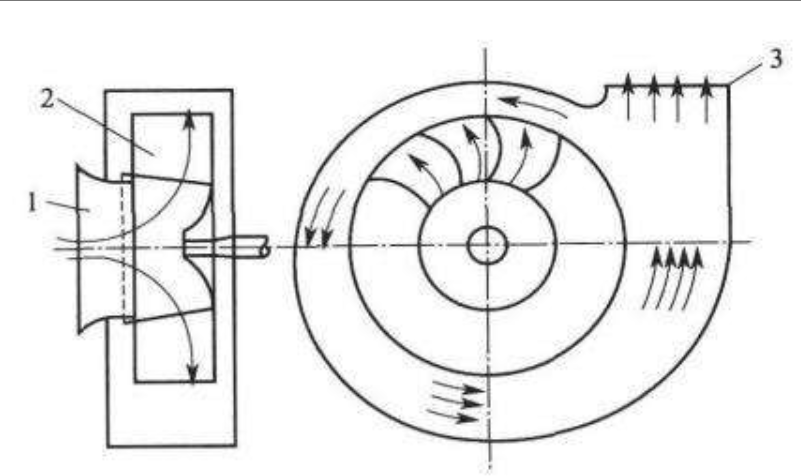
\includegraphics[width=0.5\textwidth]{images/CentrifugalFan.png}
  \caption{Centrifugal Fan Model}
  \label{fig:Centrifugal Fan Model}
\end{figure}

Centrifugal fans impart energy to the airflow by accelerating it radially outward, thereby converting rotational kinetic energy into a pressure rise. Assuming steady, incompressible flow and negligible inlet swirl velocity (\( v_{t1} = 0 \)), Euler’s turbomachinery equation gives the theoretical pressure rise as
\begin{equation}
    \Delta p = \rho u_2 v_{t2} \cdot \eta_h,
\end{equation}
where \( \rho \) is the air density, \( u_2 = \omega r_2 \) is the blade tip speed (with \( \omega \) the angular velocity and \( r_2 \) the outer radius of the impeller), \( v_{t2} \) is the tangential velocity of air at the outlet, and \( \eta_h \) is the hydraulic efficiency accounting for energy losses.

The radial component of the outlet velocity \( v_{r2} \) relates to the volumetric flow rate \( Q \) through the impeller outlet area \( A_2 \) via
\begin{equation}
    Q = v_{r2} A_2,
\end{equation}
where \( A_2 \) denotes the cross-sectional area swept by the impeller blades at the outlet.

The tangential velocity at the outlet can be approximated from blade geometry and flow conditions as
\begin{equation}
    v_{t2} = u_2 - v_{r2} \cot \beta_2,
\end{equation}
where \( \beta_2 \) is the blade outlet angle relative to the tangential direction. For backward-curved blades (\( \beta_2 < 90^\circ \)), this results in \( v_{t2} < u_2 \), contributing to higher efficiency and a more stable pressure–flow characteristic.

By substituting \( v_{r2} = \frac{Q}{A_2} \) into the expression for \( v_{t2} \), the pressure rise becomes
\begin{equation}
    \boxed{\Delta p = \rho u_2^2 \eta_h \left(1 - \frac{Q \cot \beta_2}{A_2 u_2} \right)},
\end{equation}
which explicitly illustrates the inverse relationship between pressure rise and volumetric flow rate. This negative slope of the pressure–flow curve is a key feature of centrifugal fan performance and informs system matching and control strategies.


\textbf{Validation (SRN4 centrifugal fan):}~\cite{yun1990hovercraft}
\begin{itemize}
    \item Fan radius \( R_2 = 1.75\, \mathrm{m} \)
    \item Rotational speed \( \omega = 73.3\, \mathrm{rad/s} \)
    \item Flow rate \( Q = 113\, \mathrm{m^3/s} \)
    \item Total pressure rise \( \Delta p = 5745\, \mathrm{Pa} \)
    \item Efficiency \( \eta = 0.75 \)
    \item Blade outlet angle \( \beta_2 = 45^\circ \) 
    \item Outlet width \( b_2 = 0.3\, \mathrm{m} \)
\end{itemize}

The outlet area is calculated as:
\begin{equation}
    A_2 = 2 \pi R_2 b_2 = 2 \pi \times 1.75 \times 0.3 \approx 3.30\, \mathrm{m^2}
\end{equation}

The blade tip speed is:
\begin{equation}
    u_2 = \omega R_2 = 73.3 \times 1.75 \approx 128.3\, \mathrm{m/s}
\end{equation}

The pressure rise is estimated using the momentum balance model:
\begin{equation}
    \Delta p 
    = 1.225 \times 128.3^2 \times 0.75 \left(1 - \frac{113 \times \cot 45^\circ}{3.30 \times 128.3} \right) 
    \approx 5740\, \mathrm{Pa}
\end{equation}

The experimentally measured pressure is 5745\,Pa, resulting in a relative error of approximately 0.1\%.

The required shaft power is calculated as:
\begin{equation}
    P = \frac{\Delta p \cdot Q}{\eta} = \frac{5745 \times 113}{0.75} \approx 864\, \mathrm{kW}
\end{equation}

The measured power consumption is approximately 680\,kW (subject to unit verification). The deviation may result from measurement uncertainty, actual system losses, or discrepancies in flow rate or efficiency assumptions.


\subsubsection{Physical Comparison of Fan Models}

For axial fans, the pressure rise \( \Delta p_{\text{axial}} \) scales approximately linearly with the flow rate \( Q \), i.e., \( \Delta p_{\text{axial}} \propto Q \). Consequently, the power consumption of axial fans increases quadratically with flow rate,
\[
    P_{\text{axial}} \propto Q^2.
\]
This quadratic relationship implies a rapid escalation in power demand as volumetric flow increases, making axial fans well-suited for applications requiring high flow rates but relatively low pressure rises, such as propulsion systems.

Conversely, centrifugal fans exhibit a pressure rise that decreases linearly with increasing flow rate, expressed as
\[
    \Delta p_{\text{centrifugal}} = \rho u_2^2 \eta_h \left(1 - \frac{Q \cot \beta_2}{A_2 u_2}\right),
\]
which leads to a power consumption described by a quadratic function of \( Q \) with a distinct peak:
\[
    P_{\text{centrifugal}} = \frac{\Delta p \cdot Q}{\eta} = \rho u_2^2 \eta_h \left(Q - \frac{Q^2 \cot \beta_2}{A_2 u_2}\right).
\]
This non-monotonic behavior enables centrifugal fans to deliver high pressure rises at moderate flow rates with favorable power efficiency, making them ideal for applications demanding substantial static pressure.

The simplified models capture the essential aerodynamic characteristics, providing sufficient accuracy for preliminary hovercraft lift system design and control.

\begin{table}[htbp]
  \centering
  \footnotesize
  \setlength{\tabcolsep}{4pt}
  \begin{tabular}{|l|c|c|}
    \hline
    \textbf{Aspect} & \textbf{Axial Fan} & \textbf{Centrifugal Fan} \\
    \hline
    Pressure Rise & \( \propto Q \) & \( \propto 1 - Q \)\\
    Power Consumption & \( \propto Q^2 \) & Quadratic\\
    Peak Efficiency & High rate & Moderate rate \\
    Flow & High flow & Moderate flow \\
    Pressure & low pressure & high pressure \\
    \hline
  \end{tabular}
  \caption{Core Comparison of Axial and Centrifugal Fans}
  \label{tab:fan_core_comparison}
\end{table}

Given the operational demands of hovercraft systems, lift fans require generating sufficiently high pressure rises to sustain the air cushion and support the vehicle’s weight, a requirement well fulfilled by centrifugal fans due to their efficient production of high static pressure. Propulsion fans, however, emphasize large volumetric airflow to generate thrust, a role better suited for axial fans with their capability of delivering high flow rates at lower pressure rises and with a more compact design. Hence, employing centrifugal fans for lift and axial fans for propulsion achieves an optimal compromise among aerodynamic performance, power efficiency, and mechanical simplicity, ensuring reliable and effective hovercraft operation across varied conditions.

\subsection{The Optimal Number of Fan System}
In this section, we'll determine the optimal number of both lift and propulsion fans through numerical analysis. This result will also lay a foundation for the following model.\\

In practical hovercraft designs, multiple fan arrangements are commonly used to achieve desired lift and stability. The three typical configurations are:

\begin{itemize}
  \item \textbf{Single central fan} (\(N=1\)): One large fan placed centrally under the cushion area.
  \item \textbf{Dual side fans} (\(N=2\)): Two fans placed symmetrically on either side.
  \item \textbf{Quad corner fans} (\(N=4\)): Four fans positioned near the corners of the cushion area.
\end{itemize}

These arrangements balance factors such as maximum airflow, spatial constraints, and stability.

\subsubsection{Maximum Mass Flow Rate}

Viscous losses in ducts are modeled by the Darcy-Weisbach equation:
\begin{equation}
    \Delta p_{\text{loss}} = f \cdot \frac{L}{D} \cdot \frac{1}{2} \rho v^2,
\end{equation}
where \( f \) is the friction factor, \( L/D \) the length-to-diameter ratio, \( \rho \) the fluid density, and \( v \) the mean flow velocity. For laminar flow, \( f = \frac{64}{\mathrm{Re}} \), with Reynolds number \( \mathrm{Re} = \frac{\rho v D}{\mu} \). For turbulent flow, empirical relations such as the Colebrook equation apply.

In multi-fan systems, jet interference reduces effective flow area\cite{sardoueinasab2018energy}:
\begin{equation}
    A_{\text{eff}} = A \cdot \exp(-\lambda N),
\end{equation}
where \( A \) is geometric area, \( N \) number of fans, and \( \lambda \) an empirically determined interference coefficient.

Non-uniform velocity profiles cause kinetic energy correction factor \( \alpha \geq 1 \):
\begin{equation}
    \dot{E}_{\text{kin}} = \frac{1}{2} \dot{m} \alpha v^2,
\end{equation}
with
\begin{equation}
    \alpha \approx 1 + \frac{N - 1}{4}.
\end{equation}

Fan efficiency degrades with size reduction, modeled as:
\begin{equation}
    \eta \rightarrow \eta \cdot \exp(-\beta N),
\end{equation}
where \( \beta \) depends on rotor design.

Combining these corrections, the total mass flow rate for \( N \) fans is
\begin{equation}
    \dot{m}_N = \dot{m}_1 \cdot N^{2/3} \cdot \frac{1}{\alpha} \cdot \exp\left[-(\lambda + \frac{\beta}{3})N \right],
\end{equation}
or equivalently,
\begin{equation}
    \dot{m}_N = \dot{m}_1 \cdot \frac{N^{2/3} \cdot \exp\left[-(\lambda + \frac{\beta}{3})N \right]}{1 + \frac{N - 1}{4}}.
\end{equation}

For illustration:

\begin{itemize}
  \item Single central fan (\( N=1 \)):
  \begin{equation}
      \dot{m}_1 = \left( 2 \rho^2 \eta P A^2 \right)^{1/3}.
  \end{equation}
  \item Dual side fans (\( N=2, \lambda=0.05, \beta=0.1 \)):
  \begin{equation}
      \dot{m}_2 \approx \dot{m}_1 \cdot \frac{2^{2/3} \cdot \exp(-0.117)}{1.25} \approx 1.18 \dot{m}_1.
  \end{equation}
  \item Quad corner fans (\( N=4, \lambda=0.1, \beta=0.2 \)):
  \begin{equation}
      \dot{m}_4 \approx \dot{m}_1 \cdot \frac{4^{2/3} \cdot \exp(-0.467)}{1.75} \approx 1.12 \dot{m}_1.
  \end{equation}
\end{itemize}

These examples show that moderate fan parallelization can improve mass flow despite interference and efficiency losses.

\subsubsection{Overturning Resistance and Stability}

To evaluate the system's resistance to overturning, we analyze the restoring moment \( M \) generated under a small angular perturbation \( \theta \). This moment is induced by the pressure redistribution on the air cushion and depends critically on the fan configuration. In what follows, we examine three representative layouts—namely, a single central fan, a dual-fan arrangement, and a four-fan configuration—each associated with distinct stiffness characteristics.

We begin with the simplest configuration: a single central fan (\( N=1 \)). When the platform tilts by a small angle \( \theta \), the centroid of the pressure distribution shifts horizontally by approximately \( \Delta x \approx \frac{B}{2} \theta \), where \( B \) denotes the width of the cushion. This lateral displacement generates a restoring moment of the form
\begin{equation}
    M_1 = p A \cdot \frac{B}{2} \theta,
\end{equation}
leading directly to a stiffness coefficient
\begin{equation}
    K_1 = \frac{M_1}{\theta} = \frac{p A B}{2},
\end{equation}
where \( p \) is the uniform cushion pressure and \( A \) is the total effective pressure area. Owing to its symmetry and centralized airflow, this configuration inherently provides a strong restoring torque.

To examine the effect of distributed propulsion, we next consider a dual-fan system (\( N=2 \)), with fans symmetrically placed on either side of the platform and separated by a distance \( d \). In the passive mode, the restoring effect originates from the height difference induced by gravity across the tilted cushion. This leads to a differential pressure \( \Delta p = \rho g h \theta \), where \( h \) denotes the nominal hover height and \( \rho g \) represents the hydrostatic pressure gradient. The resulting moment is given by
\begin{equation}
    M_2 = \Delta p \cdot \frac{A}{2} \cdot d = \rho g h \theta \cdot \frac{A d}{2},
\end{equation}
which yields the passive stiffness coefficient
\begin{equation}
    K_2 = \frac{M_2}{\theta} = \rho g h \cdot \frac{A d}{2}.
\end{equation}
Since typically \( \rho g h \ll p \), the passive stiffness is significantly smaller than that of the central-fan system, confirming its weaker overturning resistance.

In contrast, under active control, the fans can be modulated to impose a prescribed pressure differential \( \Delta p_{\text{active}} = k p \), where \( k \in [0,1] \) is a proportional control factor. This produces an actively induced moment
\begin{equation}
    M_2 = \Delta p_{\text{active}} \cdot \frac{A}{2} \cdot d = k p \cdot \frac{A d}{2},
\end{equation}
and the corresponding stiffness becomes
\begin{equation}
    K_2 = \frac{M_2}{\theta} = \frac{k p A d}{2}.
\end{equation}
Although still lower than the central configuration for modest values of \( k \), active control introduces the ability to dynamically enhance stiffness and stabilize disturbances. 

Note that the coefficient $k$ should be maintained within the range of  $10\%$ and $30\%$. Exceeding this threshold may result in parallel fan systems operating with significantly mismatched power capacities, consequently inducing speed loss and performance degradation, as demonstrated in the study by Chun et al~\cite{chun2011study}.

Finally, we generalize to a four-fan configuration (\( N=4 \)) arranged in a square footprint. Assuming diagonal control of opposing fans and a square base of width \( B \), the effective separation becomes \( d = \frac{B}{\sqrt{2}} \). With active pressure modulation at the same level \( \Delta p_{\text{active}} = k p \), the net restoring moment due to two diagonally opposed fans is
\begin{equation}
    M_3 = 2 \cdot \frac{A}{4} \cdot \Delta p_{\text{active}} \cdot \frac{d}{2} = \frac{k p A d}{4},
\end{equation}
and the resulting stiffness is
\begin{equation}
    K_3 = \frac{M_3}{\theta} = \frac{k p A d}{4}.
\end{equation}

In summary, centralized fan configurations deliver the highest restoring stiffness owing to concentrated pressure generation. In contrast, distributed systems sacrifice some passive stability but gain flexibility in control authority, fault tolerance, and directional thrust. Notably, active pressure regulation in multi-fan layouts can partially compensate for the reduced inherent stiffness, enabling adaptive stability management.

\subsubsection{Conclusion}

Moderate fan parallelization (\( N=2 \)) often represents an optimal compromise, improving mass flow and redundancy while keeping control complexity manageable. The choice depends on specific operational requirements, budget constraints, and maintenance capabilities.

Further quantitative optimization requires calibrated parameters
\(\lambda, \beta, k, c_0, c_1, r\) for the given application context.

\subsection{Optimal Parameter of Peripheral Jet}

As show in \ref{sec:model}, peripheral jet is the ideal model of the cross-section. 

We then want to design the optimal parameter of the peripheral jet that can take full advantage from the power given by the fixed engine. In specific, we want to design the thickness of jet at nozzle exit $t$, the inclined angle $\theta$ at the hovering height $h$ such that can minimize the total power $P_{LM}$ required for hovering the craft and resisting the drag when moving under a specific forward speed. Here we consider the movement on the ground and only consider momentum drag as we assumed before. In terms of movement on the ocean, which will be discussed in \ref{sec:wave drag}, the effect of additional drag can approach a significant small number according to a proper design. 

When analyzing a hovercraft on the ground, our model focuses only on momentum drag in terms of drag. This is because momentum drag dominates the power requirements for forward motion. Other resistances like profile drag, cushion drag, etc., are either negligible under typical ground conditions or can be accounted for within the framework of momentum drag due to their coupling effects. Additionally, momentum drag directly relates to the fundamental mechanism of airflow momentum loss during ground movement, which is crucial for optimizing the power consumption of the vehicle's propulsion system on the ground.\\
Referring to Mair's calculation about peripheral jet in the research \cite{mair1964physical}, 
we define a meaningful dimensionless parameter:
\begin{equation}
    x = \frac{t}{h} (1 + \cos\theta) \label{eq:xdef}
\end{equation}

This parameter combines the jet's geometric properties (thickness $t$, angle $\theta$) and height h into a single scaling factor, making it pivotal for optimizing the total power.

\begin{figure}[H]
  \centering
  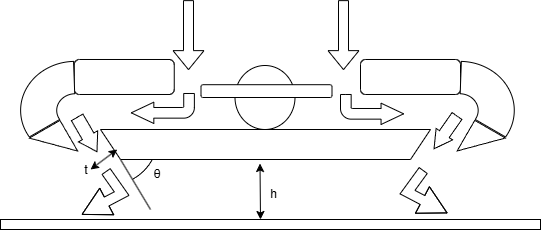
\includegraphics[width=0.5\textwidth]{images/PeripheralJet.jpg}
  \caption{Peripheral Jet}
  \label{fig:PeripheralJet2}
\end{figure}

Assume the jet is thin and with uniform static pressure equal to the mean of the cushion 
pressure and the atmospheric pressure. A formula of the relation between height of nozzle outlet above ground $h$, the cushion pressure $p_c$, mean total pressure of jet at nozzle exit $p_J$(both pressure relative to atmosphere in order to simplify the expression, i.e. comparing to former notation we use in section \ref{sec:ACM}, $p_J=H-p_0$, $p_c=p_{jet} -p_0$) and the inclined angle $\theta$ of the jet is given from \ref{sec:ACM} (\ref{eq:force_balance}):


\begin{align}
    h p_c &= J (1 + \cos\theta) \label{eq:pc} \\
    \intertext{where the momentum flux per unit length of jet $J$ derived from equation (\ref{eq:J_p0}) satisfies:}
    J &= (2p_J - p_c)t \label{eq:j} \\
    \intertext{Combining (\ref{eq:pc}) and (\ref{eq:j}) gives:} 
    \frac{p_c}{p_J} &= \frac{2t(1 + \cos\theta)}{h + t(1 + \cos\theta)} \label{eq:ratio_raw}
\end{align}



Simplifies (\ref{eq:ratio_raw}) to:
\begin{equation}
    \frac{p_c}{p_J} = \frac{2x}{1 + x}  \label{eq:thin}
\end{equation}

It should be mentioned that formula(\ref{eq:thin}) is only valid for jet with thin exit. Jones' research \cite{jones1961design} has given out a more general approximate formula that valids for both thick and thin jet:
\begin{equation}
    \frac{p_c}{p_J} = 1 - e^{-2x}  \label{eq:thick}
\end{equation}



Due to our assumption of thin jet, we use formula(\ref{eq:thin}) for the following calculation.

Theoretical hovering power $P_L$ is derived from energy conservation:
\begin{equation}
    P_L = p_J Q \quad 
\end{equation}
The total volume flow per unit time in lifting jets $Q$ can be calculated by:
\begin{equation}
    Q = C \cdot t \cdot v_{\text{jet}}  
\end{equation}
where $C$ is the perimeter of the craft measured at nozzle exit, $t$ is the thickness of nozzle exit and $v_{\text{jet}}$ is the gas speed of jet at nozzle exit.

Meanwhile, $v_{\text{jet}}$ can be calculated through Bernoulli equation:
\begin{equation}
    v_{\text{jet}} = \sqrt{\frac{2(p_J-p_c)}{\rho}}
\end{equation}
    Substituting $t = \dfrac{x h}{1 + \cos\theta}$ from (\ref{eq:xdef}) and $p_J = \frac{1 + x}{2x} p_c$ from (\ref{eq:thin}):
\begin{equation}
    P_L = \frac{C h p_c^{3/2}}{2 \rho^{1/2} (1 + \cos\theta)} \left( \frac{1 + x}{x^{1/2}} \right) \label{eq:p0}
\end{equation}


Take dimensionless parameter:
\begin{equation}
K' = \frac{Chp_c^{3/2}}{2\rho^{1/2}(1 + \cos \theta)}
\end{equation}

we have:
\begin{equation}
    P_L = K' \left( \frac{1 + x}{x^{1/2}} \right)
\end{equation}

At craft's forward speed $v_f$ , dynamic pressure $q$ can be calculated through Bernoulli equation:
\begin{equation}
    q = \frac{1}{2} \rho v_f^2
\end{equation}

Power needed to overcome momentum drag is given by: 
\begin{equation}
    P_M = 2 q Q \label{eq:pm} 
\end{equation}

Further considering the lifting fan power saved by ram effect $qQ$,
the total required power is:
\begin{equation}
    P_T = P_L + P_M -qQ
    = K' (\frac{1 + x}{x^{1/2}}) ( 1 + \frac{2 k x}{1 + x} )
\end{equation}
where: 
\begin{equation}
    k = \frac{q}{p_c}
\end{equation}



In order to take full advantage of the fixed power, $P_T$ should be minimized, thus it satisfy:
\begin{align}
    &\frac{\partial P_{T}}{\partial x}= 0 \\
    \text{i.e.} \quad&\frac{\partial}{\partial x} \left[ \left( \frac{1 + x}{x^{1/2}} \right) \left(1 + \frac{2 k x}{1 + x} \right) \right]= 0
\end{align}

Solving yields:
\begin{equation}
    \boxed{ x_{\text{opt}} = \frac{1}{1 + 2k} } \label{eq:xopt}
\end{equation}

Through the data of different type of hovercraft, we can verify whether the $x_{opt}$ satisfy the thin jet condition.

\begin{table}[h]
\centering
\caption{Thin Jet Verification}
\begin{tabular}{lllll}
\toprule
\textbf{Name} & \textbf{Speed (m/s)} & \textbf{Pressure (Pa)} & \textbf{$x_{opt}$} \\
SRN 6 & 30.87 & 1480 &  0.558 \\
BH 7 & 33.45 & 2200 &  0.617 \\
SRN 4 & 36.02 & 2400 & 0.601 \\
N300 & 31.90 & 2000 & 0.616 \\
\end{tabular}
\label{tab:thinjet}
\end{table}


As shown in table \ref{tab:thinjet}, the $x_{opt}$ is around 0.6, at which (\ref{eq:thin}) performs well and the assumption of thin jet make sense.

\begin{figure}[H]
  \centering
  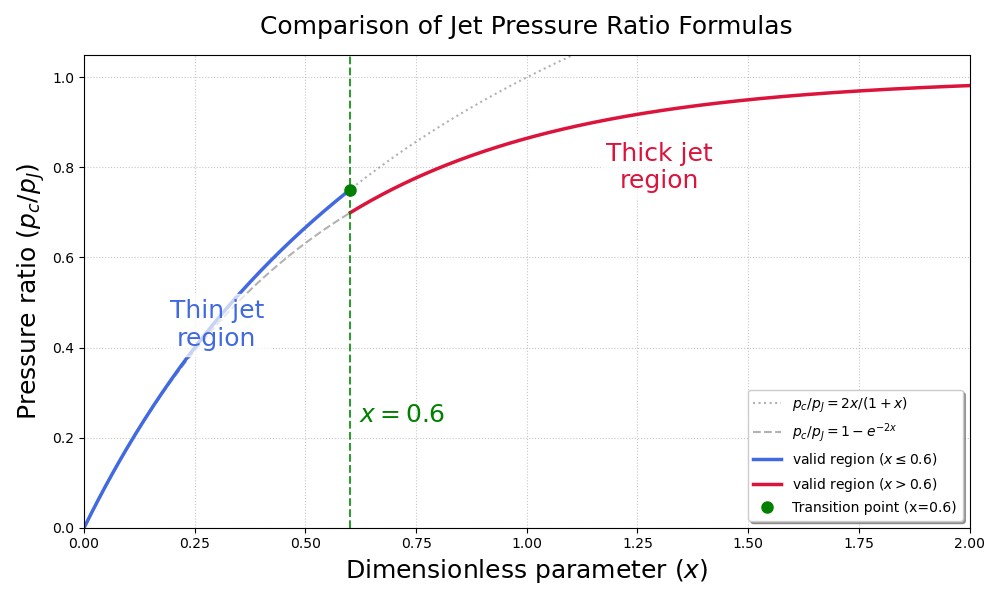
\includegraphics[width=0.5\textwidth]{images/compare.png}
  \caption{Comparison of Jet Pressure Ratio}
  \label{fig:compare}
\end{figure}

\subsection{Minimize Wave Drag}
\label{sec:wave drag}
In this section, we consider hovercraft's movement on the ocean. In ocean hovercraft modeling, we focus solely on wave drag as the new resistance term because it dominates energy loss at critical speeds (e.g., hump speed) due to free-surface wave generation—uniquely tied to water dynamics. Other drag components (e.g., friction) are either negligible or already addressed in baseline models, while wave drag’s direct link to cushion pressure and hull geometry enables essential design optimization for efficiency. Our goal in this section is to design the hovercraft in order to minimize the effect of wave drag to be a significant small number that can be neglected.

When craft moving on the ocean, we can calculate the wave drag through equations (\ref{eq:sigma})(\ref{eq:froude})(\ref{eq:R}) given by Crewe's research\cite{crewe1960hovercraft}

The shape of water surface depends on

\begin{equation}
\sigma = \frac{p_{c}}{\rho_{w}gl} \label{eq:sigma}
\end{equation}

and Froude number 
\begin{equation}
F = \frac{v_f}{\sqrt{lg}} \label{eq:froude}
\end{equation}

The shape change of water causes wave drag $R$, which satisfies:

\begin{equation}
\frac{R}{\sigma mg} = 2\left[1 - \cos\left(\frac{1}{F^{2}}\right)\right] \label{eq:R}
\end{equation}

Without considering the change of mass $m$, increasing $l$ leads $\sigma$ to decrease, which further decrease wave drag $R$. So if $m$ can be controlled properly, having a hovercraft with larger cushion length $l$ can be a good choice to minimize the wave drag.

However, in practice, $m$ may increase proportionally with $l$, so normalized wave drag $\frac{R}{\sigma mg}$, which is used to indicate the effect of wave drag regardless of the scale of the craft, is a more proper expression to optimize when minimizing the effect of wave drag.

$\frac{R}{\sigma mg}$ is strongly related to Froude number $F$, and $F$ can be controlled by both $V$ and $l$ as shown in (\ref{eq:R})

Since the power $P_0$ is given by the single engine, we can obtain the expression of $V$

\begin{align}
\quad&P_0 = P_T \\
&= K'\left[ \frac{1+x}{x^{1/2}} \right] \left[ 1 + \frac{2kx}{1+x} \right] \\
&\text{When} \quad x = x_{\mathrm{opt}} = \frac{1}{1+2k} \\
&P_0 = 2K'\sqrt{1 + 2k} \\
&\Rightarrow k = \frac{1}{2} \left( \frac{P_0^2}{4K'^2} - 1 \right) \\
&\text{Since} \quad k = \frac{q}{p_c} = \frac{\frac{1}{2}\rho v_f^2}{p_c} \\
&\text{we have} \quad v_f = \sqrt{ \frac{p_c}{\rho} \left( \frac{P_0^2}{4K'^2} - 1 \right) } \label{eq:V}
\end{align}

By changing cushion length $l$, $F$ can be changed to obtain a small $\frac{R}{\sigma mg}$.

Suppose we want
\begin{equation}
\frac{R}{\sigma mg} \leq \varepsilon  
\end{equation}
and it's change is not critical when $F$ changes, 

\begin{figure}[H]
  \centering
  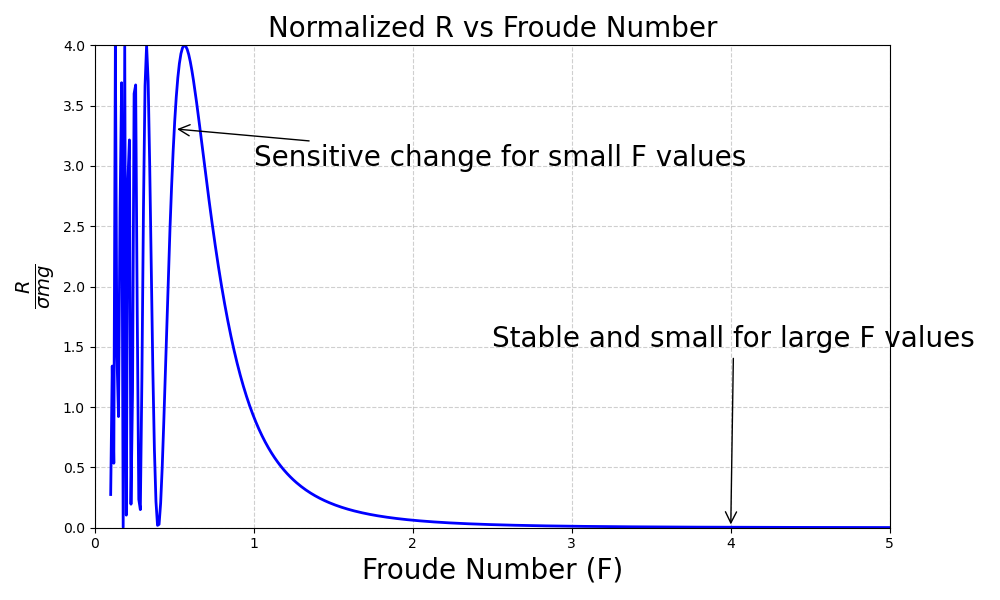
\includegraphics[width=0.5\textwidth]{images/R.png}
  \caption{Wave drag's function about Froude number}
  \label{fig:R}
\end{figure}

Observing figure ~\ref{fig:R}, when $F$ is small($F\in(0,1)$),  $\frac{R}{\sigma mg}$ changes critically as F has a small change. And when $F$ becomes large, $\frac{R}{\sigma mg}$ becomes small and stable. So larger $F$ performs better when finding small enough 

\begin{equation}
\frac{R}{\sigma mg} \leq \varepsilon 
\end{equation}

Then, we have

\begin{equation}
F^{2} \geq \frac{1}{\arccos\left(1 - \frac{\varepsilon}{2}\right)} \Rightarrow \frac{v_f^{2}}{lg} \geq \frac{1}{\arccos\left(1 - \frac{\varepsilon}{2}\right)}
\end{equation}

\begin{equation}
\Rightarrow l \leq \frac{v_f^{2}}{g} \frac{1}{\arccos\left(1 - \frac{\varepsilon}{2}\right)}
\end{equation}

Substitute $v_f$ by (\ref{eq:V})
\begin{equation}
 \boxed{l \leq \frac{p_{c}}{\rho g} \left( \frac{1}{4 K^{\prime 2}} P_{0}^{2} - 1 \right) \frac{1}{\arccos \left( 1 - \frac{\epsilon}{2} \right)} }
\end{equation}

\subsection{The position of Two Fans}
In this section, we'll discussion the optimal position of two fans in terms of the stability of the hovercraft. In this condition it means the conservation of angular momentum in stable voyage, meaning that the torque is 0 when the external force is 0. After that, we'll take both the passengers comfort and cost into consideration to decide the optimal design\\
\begin{enumerate}
    \item he shape of the hovercraft from side view is two semi-circles with one rectangle, where the front and tail of the hovercraft is two semi-circles
    \item the position of COM is the geometric center of the hovercraft
    \item the horizontal distance between propulsion fan and COM is $\frac{L}{2}$, meaning it locates at the very tail of the hovercraft to maximum the space utilization rate before the fan
    \item  The mass of the fan is negligible
    \item The total friction on the hovercraft can be equivalent to a force on COM
    \item The lifting force $F_1$ and propulsion force $F_2$ is fixed during the movement
\end{enumerate}


Based on the conclusion from the previous chapter, the top view and side view should look like the following figures, with the relevant parameters noted besides. 

\begin{figure}[H]
  \centering
  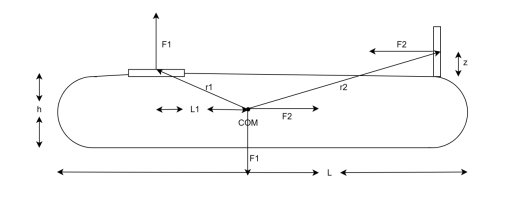
\includegraphics[width=0.5\textwidth,height=0.3\textwidth]{images/TopView.jpg}
  \caption{Side View}
  \label{fig:Side View}
\end{figure}

\begin{figure}[H]
  \centering
  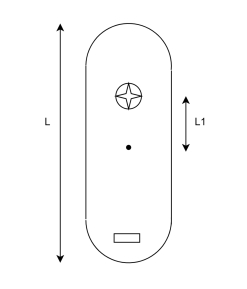
\includegraphics[width=0.5\textwidth,height=0.45\textwidth]{images/SideView.jpg}
  \caption{Top View}
  \label{fig:Top View}
\end{figure}



First, we can decide the ratio of $L_1$ and $z$ with the equilibrium of torque where the hovercraft reaches the equilibrium of force, as indicated in Figure 6, where we choose COM point as reference point.
\begin{equation}
r_1 \times F_1 = r_2 \times F_2
\end{equation}
After plugging in the parameters in Figure 6, we get 
$(\frac{h_1}{2}+z)*F_2=L_1*F_1$
Since $F_1$ and $F_2$ is known, we can express $L_1$ by $z$ using the equation
\begin{equation} 
L_1=(\frac{h_1}{2}+z)*\frac{F_2}{F_1}
\end{equation}
This equation shrinks the number of variables from 2 to 1.\\

Next we'll consider the comfort of the passenger in terms of the amplitude of sound, which, in this model, is simplified to the decibel at COM, thus deciding the optimal choice of $z$.\\
The typical decibel of fan at distance $r_0=1m$is given by \textit{Sound and Vibration DESIGN AND ANALYSIS}~\cite{national1994sound}:
\begin{equation} 
 L_0 = K_w + 10 \log_{10} \left[ \frac{Q_f}{Q_1f} \right] + 20 \log_{10} \left[ \frac{P_f}{P_1f} \right] + C
\end{equation}
where:

\begin{itemize}
\item $L_0$ = estimated sound power level (dB) of the fan
\item $K_w$ = specific sound power level (dB) from
\item $Q_f$ = the fan flow rate (L/s)
\item $Q_1f$ = reference flow rate (0.47 L/s)
\item $P_f$ = fan total pressure (Pa)
\item $P_1f$ = reference pressure (0.249 Pa)
\item $C$ = correction factor (dB) for the case where the point of fan operation is other than the point of peak efficiency. 
\end{itemize}

So $L_0$ is a fixed number as long as the pressure is fixed, which has been proven in the previous section.
Since amplitude is proportional to the inverse of the square of distance, namely $I \propto \frac{1}{r^2}$, the relationship of decibel and distance $r = \sqrt{(\frac{L}{2})^2+(\frac{h_1}{2}+z)^2}$ is given by:
\begin{equation} 
L_{COM} = L_0 - 20 \log_{10}\left(\frac{r}{r_0}\right)
\end{equation}

According to the research published by \textit{Noise}~\cite{kahneman2021noise}, the height decibel people can bear in a comfort zone is 60 dB, so $r \geq 10^{\frac{L_0 - 60}{20}}$. Considering both the cost and the friction of wind, $z$ should be as small as possible in the acceptable scope.
\[
z =
\begin{cases}
-\dfrac{h_1}{2} + \sqrt{10^{\frac{L_0 - 60}{10}} - \dfrac{L^2}{4}}, & \text{if } 10^{\frac{L_0 - 60}{20}} > \sqrt{\left(\dfrac{L}{2}\right)^2 + \left(\dfrac{h_1}{2}\right)^2} \\
0, & \text{otherwise}
\end{cases}
\]






\section{Discussion}
\subsection{Discussion of the Result}
The optimization results for the amphibious air cushion vehicle (ACV) design are highly reasonable and carry significant practical value. The systematic, seven-step approach ensures each design element is rigorously evaluated, building a cohesive and efficient system. The prioritization of stability and energy efficiency aligns with the operational demands of maritime environments, where dynamic conditions require robust solutions. The application of air cushion mechanics to guide design choices is theoretically sound, leveraging established principles to ensure reliable performance. The fan selection and positioning strategy reflects a practical balance, optimizing power use while minimizing operational disturbances like noise, which is critical for real-world usability. The derived parameters and cushion length constraints demonstrate a nuanced understanding of environmental interactions, such as wave drag, ensuring the design’s adaptability and efficiency. These results are not only logically consistent but also practically significant, offering a scalable framework for ACV development that enhances performance in challenging conditions, reduces energy costs, and informs future engineering efforts in similar domains.

\subsection{Discussion of the Model}

\subsubsection{Ideal Model of the Cross-section of
Hovercraft}

\textbf{Strength:} this model based on two existing models, which have already stood the test of time, managing to eliminate other bad models and considerably simplify the analyzing process. Also, this cross-section analysis is independent of other parts, which enable us to control the variables and create a solid foundation for further analysis.\\
\textbf{Weakness:} The model treats the hovercraft’s side wall as a short pipe, which oversimplifies the complex geometry of the Peripheral Jet’s curved structure. This simplification may fail to capture localized turbulence or pressure gradients in the intricate airflow paths, leading to discrepancies between theoretical flow rates and actual performance.\\

\subsubsection{Air Cushion Model}

\textbf{Strengths:} The model is theoretically sound, and the resulting trends of the calculated curves align well with empirical formulas and experimental data, with deviations remaining within reasonable margins of error.

\textbf{Weaknesses:} The model relies on several simplifying assumptions that may not hold in practical scenarios, particularly regarding the interactions between airflow streams from different fans, which are treated as non-interfering.

\subsubsection{Comparative Modeling of Centrifugal and Axial Flow Fans}

\textbf{Strengths:} The model effectively captures and explains the characteristic differences between axial and centrifugal fans.

\textbf{Weaknesses:} The blade element model, while commonly used in practical estimations through iterative methods, lacks accuracy when applied as a purely theoretical model due to its reliance on empirical fitting and simplifications.

\subsubsection{Optimal Fan System Model}

\textbf{Strengths:} The model provides a rational explanation for the industry's selection of different fan systems based on specific operational goals. It successfully illustrates how system configurations are optimized according to performance trade-offs.

\textbf{Weaknesses:} The key governing equations are heavily dependent on experimental fitting, which may limit their universality across different design scenarios. Moreover, the weighting and comparison of multiple performance variables involve subjective judgments, potentially affecting the objectivity of the optimization process.



\subsubsection{Optimal Parameter of Peripheral Jet}
\textbf{Strength:}In this section, we show peripheral jet's optimal geometry features that can take full advantage of the given power. Furthermore, since the optimized parameter is dimensionless, this single scaling factor can be used to design jets for hovercrafts in different scales.\\
\textbf{Weakness:}The result demands thin jet assumption, which is not accurate when the jet exit is thick.\\
\subsubsection{Minimize Wave Drag}
\textbf{Strength:} This model considers hovercraft's movement on the ocean. Controlling the length of cushion to make the effect of wave drag significantly small.\\
\textbf{Weakness:}Under some conditions, the cushion length is required to be large enough for huge hovercrafts, where the effect of wave drag can't be ignored and the model is invalid.\\
\subsubsection{The position of Two Fans}
\textbf{Strength:} this model manages to integrate both the physical analysis with passengers' actually feeling in the optimization process, which can provide a realistic reference for the actual condition. Further, this model parameterizes the height of propulsion fan and the distance of lift fan, offering an analyzing and detailed parameters for the location of fan. This parameterization outperforms the method of comparing several discrete models, aiming to reach a continuous prediction.\\
\textbf{Weakness:} this model only considers the condition when the hovercraft is on balanced voyage with external force is zero. However, in most situation, there will be disturbance during voyage, which can not directly derive from this model. Also, The sound power level $( L_0 = K_w + 10 \log_{10} \left[ \frac{Q_f}{Q_1f} \right] + 20 \log_{10} \left[ \frac{P_f}{P_1f} \right] + C) $assumes fixed fan parameters. However, fan flow rate  and pressure may vary with operating conditions. The model does not account for these variations, potentially underestimating the complexity of noise.\\
\section{Conclusion}

This study on optimizing hovercraft design for amphibious air cushion vehicles (ACVs) with fixed power yields significant findings. Basically, this optimization process is decomposed into seven incremental parts, each of the part is optimized independently or based on the previous result to  reach a global optimization.

The peripheral jet configuration was identified as the optimal cross-sectional design, offering superior stability and energy efficiency compared to the plenum chamber model, particularly in maritime conditions with wave-induced vibrations. Then the principles of air cushion mechanics are studied, serving as a compelling tool to predicting lifting force and optimizing skirt configuration, whose accuracy has been verified by data. After that, by comparing the pros and cons of centrifugal and Axial flow fans, it can be concluded that centrifugal fan is suitable for high $p_c$, low flow rate while Axial fan is the opposite. Then the best number of fans are taken into consideration, resulting in 1 propulsion fan and 1 lift fan.  In the next part, based on the model of cross-section that has been proven to be ideal, the optimal parameters are determined to maximize the usage of fixed power, where $x_{opt}$ is the optimal parameter from calculation. After that, the additive wave drag is considered when the hovercraft is on ocean. To minimize this drag and boost efficiency, the optimal length of cushion $l$ is calculated, which should lie on a certain range, specifically, $l \leq \frac{p_{c}}{\rho g} \left( \frac{1}{4 K^{\prime 2}} P_{0}^{2} - 1 \right) \frac{1}{\arccos \left( 1 - \frac{\epsilon}{2} \right)}$. Finally, based on the specific number of fan, optimal fan positioning is calculated by balancing torque and minimizing decibel at the position of COM, leading to optimal height $z$ and distance $L_1 = (\frac{h}{2} + z)\times \frac{F_2}{F_1}$.
\bibliography{references}

\newpage
\onecolumngrid
\appendix 

\section{Code}


    \begin{figure}[h]
        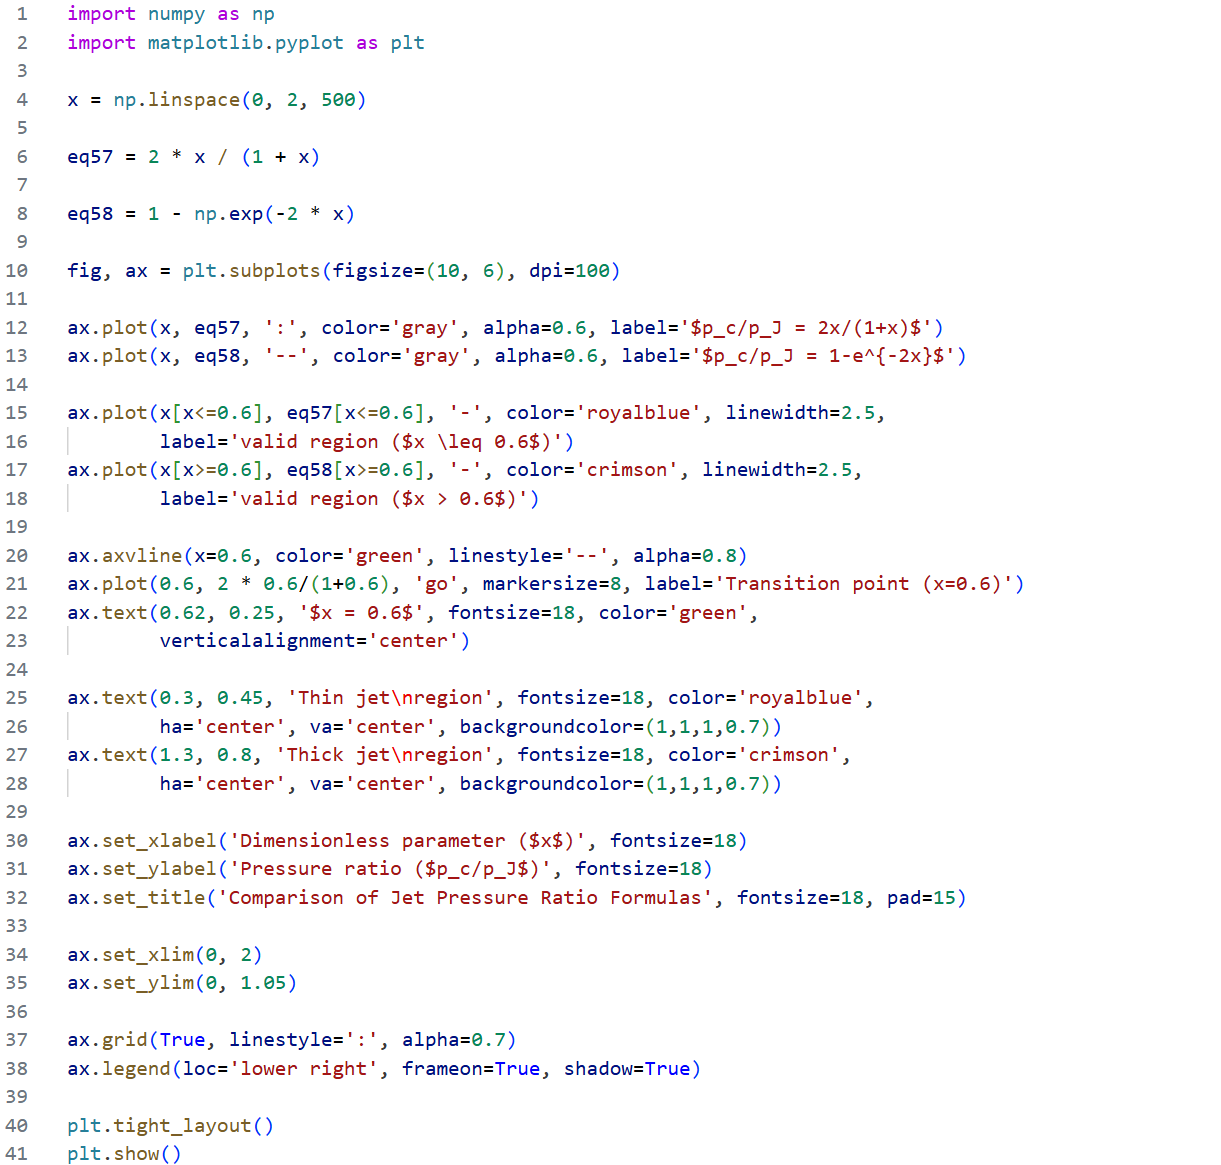
\includegraphics[width=\textwidth, height=0.8\textheight]
        {images/plotCompare.png}
    \end{figure}



    \begin{figure}[h]
        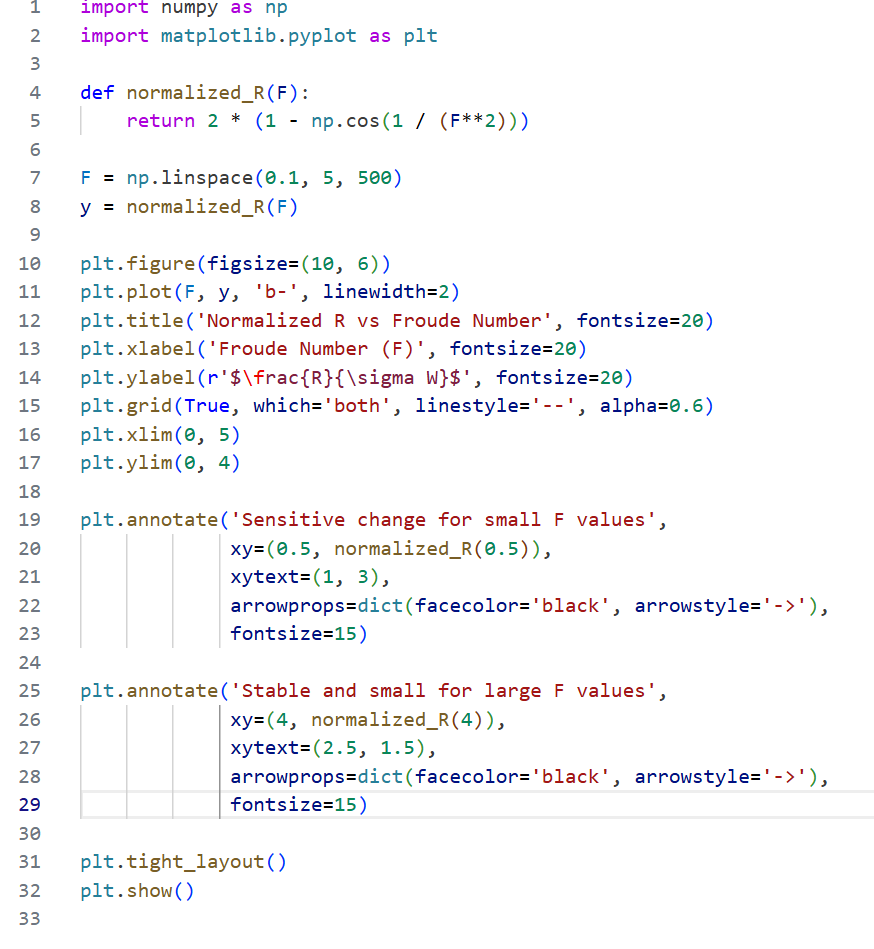
\includegraphics[width=\textwidth, height=0.8\textheight]
        {images/plotR.png}
    \end{figure}


\end{document}

